\chapter{Approach}
\label{chapter3}
\thispagestyle{empty}

\section{Dynamic Binary Instrumentation}
\paragraph{}
Dynamic Binary Instrumentation is a technique for analysing the behaviour of a binary application through the injection of instrumentation code. The instrumentation code can be developed in an high level programming language and is executed in the context of the analysed binary with a granularity up to the single assembly instruction. The injection of instrumentation code is achieved by implementing a set of callbacks provided by the \ac{DBI} framework. The most common and useful callbacks are:
\begin{itemize}
 \item Instruction callback: invoked for each instruction
 \item Image load callback: invoked each time an image (dll or Main image) is loaded into memory
 \item Thread start callback: invoked each time a thread is started
\end{itemize}
Besides the callbacks the \ac{DBI} framework allows to intercept and modify operative system \acp{API} and system calls and this is very useful to track some behaviours of the binary, like the allocation of dynamic memory areas.

\section{Approach overview}
\paragraph{}
Our tool exploits the functionalities provided by the Intel PIN \ac{DBI} framework to track the memory addresses which are written and then executed with an instruction level granularity.
More in details for each instruction the following steps are performed:
\begin{enumerate}
\item Instruction Filtering: ignore the effects of a particular set of instructions for performance reasons
\item Written addresses tracking: keep track of each memory address which is written in order to create a list of memory ranges of contiguous writes defined \textit{Write Intervals} 
\item \textit{\ac{WxorX}} instructions tracking: check if the currently executed instruction belongs to a \textit{Write Interval}. This is a typical behaviour in a packer that is executing the unpacked layer and for this reason we trigger a detailed analysis which consists of:
	\begin{enumerate}
	\item Dumping the main image of the \ac{PE} and a memory range on the heap depending on the address of the current instruction
	\item Reconstructing the \ac{IAT} and generating the correct Import Directory
	\item Applying some heuristics to evaluate if the current instruction is the \ac{OEP}
	\end{enumerate}
\end{enumerate}
The result of our tool is a set of memory dumps or reconstructed \acp{PE} depending on the result of the \ac{IAT} fixing phase and a report which includes the values of each heuristic for every dump. Based on these information we can choose the best dump, that is the one that has the greatest chance of work.

\section{Approach details}
\paragraph{}
In this section we are going to describe in details the steps introduced in the previous section.
\paragraph{}
During the development we have adapted our approach in order to increase speed and effectiveness of our tool. Following there is a detailed explanation of our improvements on the initial approach:
\begin{enumerate}
\item in the first step, we add the option of not to track writes of library instructions on the stack and in the \ac{TEB}
\item in the second step we filter instructions of known libraries before dumping
	\begin{enumerate}
	\item when trying to reconstruct the \ac{IAT} we added some code in order to deal with 			obfuscation techniques like \textit{\ac{IAT} Redirection} and \textit{Stolen \ac{API}}
	\item we implemented five heuristics:
		\begin{itemize}
		\item entropy: check if the value of the entropy is above a certain threshold
		\item long jump: check if the "distance" between the current EIP and the previous 			one is above a certain threshold
		\item jump outer section: check if the current EIP is a different section from the 		one of the previous EIP
		\item pushad popad: check is a \textit{pushad-popad} pattern has been found in the trace
		\item init function calls: check if the imports of the dump are functions commonly 			 used by the malware and not by the unpacking layers
		\end{itemize}
	\end{enumerate}
\end{enumerate} 
For the instructions that execute from the same write set we adopted the following approach: if the "distance" between the current EIP and the EIP of the previous instruction is above a given threshold then we do the same as if we were in the case 2, otherwise we jump to the next instruction.\\
Finally, we have noticed that dumping only the main executable in memory is not enough because some packers dump the final payload on the heap. In order to deal with it, we track heap allocations and writes inside an heap interval. If necessary, we dump these intervals too.

\subsection{Instructions filtering}
\paragraph{}
Since our tool works with an instruction level granularity, limiting our analysis to the relevant instruction of the program is a critical point. For this reason we have introduced some filters, based on the common behaviours showed by the packers, which make our tool ignore the effects of a set of instructions. More in detail two kind of instructions are not tracked by default:
\begin{itemize}
	\item Write instruction on the \ac{TEB} and on the Stack
	\item Instruction executed by known Windows Libraries
\end{itemize}
The write instructions on the stack are ignored because unpacking code on the stack is not common compared to unpacking it on the heap or inside the main image. Moreover many instructions write on the stack and keeping track of all the written addresses would downgrade the performances gaining little advantages against a very small set of packers.\\
The same considerations can be applied to the instructions which write on the \ac{TEB}, since most of these writes are related to the creation of instruction handlers and there is very little chance that a packer uses this addresses to unpack the encrypted payload.\\
The instructions executed by known Windows Libraries are never considered when checking if the current instruction address is contained inside a \textit{Write Interval} because this would mean that the packer writes the malicious payload in the address space of a know Windows Library. This behaviour has never been identified in the packer analysed; moreover, this could introduce some crashes if the application explicitly use one of the functions which have been overwritten.

\subsection{Heuristics description}
\paragraph{}
Our tool makes a dump each time the \ac{WxorX} law is broken in a new \textit{Write Interval} or in an existing one if \textit{InterWriteSet} analysis is enabled. Consequently, at the end of the execution we may have a lot of dumps and check them manually can be very time-consuming. Heuristics help in automatically identify the dumps that are most likely to work and also provide a "best dump", the one with the greatest chance to be the contain the original unpacked code. All the heuristics are described in \cite{Practical_Malware_Analysis}.
\paragraph{}
Entropy can be considered as a measure of the disorder of a program. For example, random data have the highest possible entropy. Since encrypted data more closely resembles random data, entropy can be used in detecting if an executable has been compressed, encrypted or both. Usually compressed files have less entropy that the original files, because the purpose of compression is to reduce the dimension of the file preserving some patterns used to recover the information. Encryption, on the opposite, has the goal of making unreadable a file, that is ideally changed in a random stream of bits. For example:\\
FFFFFFFFFFFFFFFFFFFF --------\textgreater 20'F' (compressed)\\
FFFFFFFFFFFFFFFFFFFF --------\textgreater ;LAKSDFJA;WIEFEJ;AEJF (encrypted)\\
As a result, while decompressing a file, its entropy slightly increase; while decrypting a file, its entropy slightly decrease. Consequently, in order to identify that a decompression or a decryption stage is finished, we have to check the absolute value of the difference between the initial and the current entropy.
\paragraph{}
It is very uncommon that the unpacking stub is located just under or above the \ac{OEP}. Instead, once the original code is fully unpacked, there is a long jump from the unpacking stub to the \ac{OEP} of the unpacked code. Sometimes, this jump has the target address is in a completely different section from the start address. This technique is called \textit{tail jump} and may be a sign of the completion of an unpacking stage. 
\begin{figure}[!ht]
	\begin{center}
   		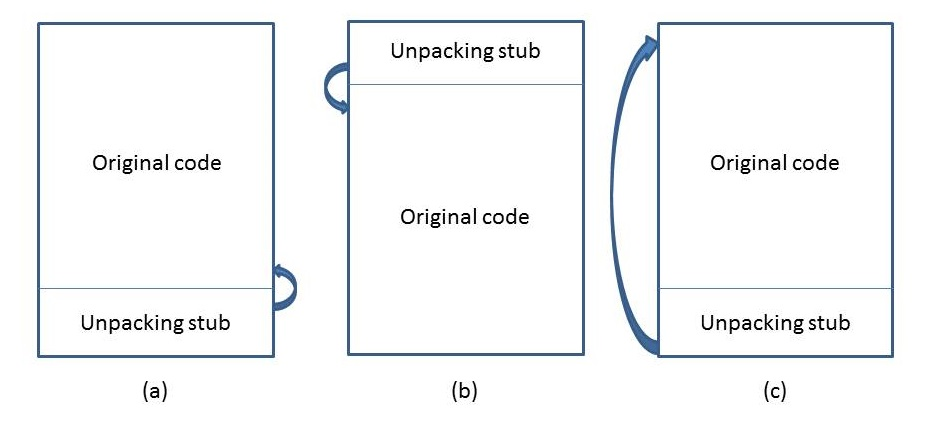
\includegraphics [width=\textwidth]{./pictures/Original Code And Unpacking Stub.jpg}
	\end{center}
	\caption{Different jumps from the unpacking stub to the original code}
	\label{Original Code And Unpacking Stub}
\end{figure}
In Figure \ref{Original Code And Unpacking Stub}, the cases (a) and (b) are extremely rare, while case (c) is the most common.\\
We base on these considerations the \textit{long jump} and \textit{jump outer section} heuristics.
\paragraph{}
Usually packers employ a technique called \textit{pushad-popad}. The \textit{pushad} function stores on the stack the values of all the registers and the \textit{popad} function restores them in the registers. After a \textit{pushad}, a packer can execute its unpacking routine and soon before the \textit{tail jump} it can restore all the registers with a \textit{popad}. In this way, the two instructions almost delimit the unpacking stub and help to identify the range of memory addresses in which the \ac{OEP} is located. As an example, a commercial packer like \textit{ASPack} employs this technique.
\paragraph{}
When a malware is packed, it usually exhibits very few or false imports. This is a technique of obfuscation used by some packers in order to hide the real behaviour of the malware. Of course, it is a job of the packer to fully reconstruct the \ac{IAT} in order to make the binary runnable.\\
The purpose of the \textit{init function calls} heuristic is to search in the \ac{IAT} for functions commonly used by the malware and not by the unpacking stub. For example, if a malware has to contact an Internet domain to download some malicious code, it will have in its imports some internet communication \acp{API} like \textit{connect} and \textit{send}. Since the unpacking stub does not need them to perform its job, when packed the binary will not have these \acp{API} in its \ac{IAT}, but the packer will take care of inserting them among the imports during the unpacking stage. In some extreme cases, the packed binary may have as imports only the \textit{GetProcAddress} and \textit{LoadLibrary} functions, because these two are used to dynamically load libraries and functions.\\
Consequently, once identified some "interesting" \acp{API} for the malware but not for the packer, we check how many of them a dump has among its imports. Usually, the more of them, the higher the probability of being the correct dump.
\paragraph{}
\subsection{Evaluation of \textit{InterWriteSet} analysis}
\paragraph{}
The initial approach was to dump the code and trigger the analysis of if once the \ac{WxorX} law was broken in a \textit{Write Interval} for the first time and then ignore all the subsequent instructions from the same \textit{Write Interval}. However, when analysing a binary packed with \textit{mpress}, we noticed the behaviour in Figure \ref{mpress behaviour} that forced us to slightly modify the initial approach.\\
\begin{figure}[!ht]
	\begin{center}
   		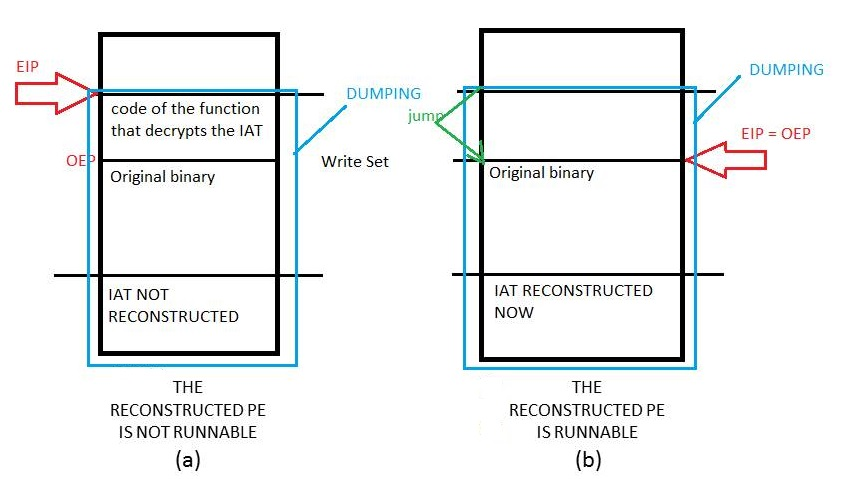
\includegraphics [width=\textwidth]{./pictures/InterWriteSet Analysis - mpress.jpg}
	\end{center}
	\caption{Mpress behaviour}
	\label{mpress behaviour}
\end{figure}
When \textit{mpress} enters for the first time the \textit{Write Interval} which contains the original code (a), it jumps in an area of memory that contains a small stub that reconstructs the \ac{IAT} and then jumps to the original code (b), that resides in the same \textit{Write Interval}. With the original approach we were able to dump the code in (a), but we ignored the jump in (b) and so we were unable to recreate a running \ac{PE}.\\
Consequently, we adapted our approach to deal with this behaviour: we consider jumps inside the same \textit{Write Interval} only if they are longer than a given threshold. If this is the case, we trigger the analysis as if it was the first time the \ac{WxorX} law is broken. However, this improvement may potentially generate too many dumps, making the analysis very slow and difficult. For this reason there is a maximum number of jumps that are considered inside the same \textit{Write Interval}.